%%------------------------------------------------------
%  
%  Evaluation include for dissertation
%
%------------------------------------------------------

Why write in first person in this chapter?

Burrows et al. (2000) suggest that writing in a reflective style enhances the
author's learning\cite{JEE:JEE657}. Coombs (2001) identified introspection and
mindfulness as habits of mind to promote reflection. Writing in the first
person reflects such introspection\cite{coombs2001reflective}.

\section{ Achievements \& Impact}

Partridge was conceptualised as a tool to assist with scientific research on
the world wide web by learning the preferences of researchers and returning
sets of papers that might interest them. Although it does not yet provide an
automated solution to `information overload' in the form of a suggestion
engine, Partridge goes a long way towards demonstrating the feasibility of such
a system and already serves as an elegant search tool for filtering out a great
deal of irrelevant literature.

\subsection{ Paper Preprocessor}

One of the biggest achievements in the development of Partridge is the flexible
and resilient paper preprocessing module. This was the most difficult part of
the system to build and a great deal of time was spent building the various
converters and classifiers that make up the 1236 lines of code that went into
the module. Some of the challenges encountered (see below) during the
implementation of the paper processor served as greatly valuable lessons in
working with artificial intelligence systems. 

During the development of the paper processor, I felt that I learnt the most
from building the paper type classifier. The implementation of the classifier
was not difficult in itself. However, determining which features to use for the
classifier and the clustering analysis were entirely new concepts to me and
required a lot of investigative work and reading to help me to understand the
processes and how they should be applied.

Working with the Python implementation of SAPIENTA demonstrated the importance
of machine learning evaluation methods for testing classifiers rather than
making assumptions about `sensible looking' output. When the application was
run on a set of papers acquired for Partridge's corpus, it seemed to give
sensible CoreSC classifications for the papers. However, upon further analysis
and calculation of Python SAPIENTA's Classifier Accuracy, it was determined
that the system was only getting 44\% of CoreSC annotations correct, an
unacceptably low success rate. If I hadn't have run the evaluation functions on
SAPIENTA, it would have been easy to assume that it was correctly classifying
the papers, tainting the input papers and potentially disrupting the
investigation into CoreSC makeup and paper type.


\subsection{User Interface}
The Partridge user interface is also a great success, providing a highly usable
and intuitive representation of the relatively complicated processes that are
used to classify and organise the papers. The use of HTML and JavaScript
interactive elements instead of static pages and synchronous calls to the web
server was certainly a good idea, providing a modern system that keeps the user
informed at all times. The decision to use the jqBBQ library to add browser
history support further enhanced the user experience, allowing users of
Partridge to share links to specific search results over social media channels
and potentially bookmark significant results.

I was particularly pleased with the Bookmarklet which makes adding papers to
Partridge significantly easier for non-authors and those who are unsure about
licensing and copyright restrictions on the papers in the corpus. The
bookmarklet was quite difficult to implement, requiring parsers for each of the
supported journal sites. However, I think it offers the most significant
improvement-to-time-invested ratio of any feature in the project.

The project's impact can also be considered a great achievement, with interest
from a growing user-base and some of the larger open access journals whose
papers are interested by the system.

\subsection{Professional Development}

One of the skills that I have honed through my dissertation project this year
has been reflecting communally upon my work with my supervisors. During my work
placement at IBM, I was loosely supervised, however it was never to the close
and exacting standards of Dr Clare and Dr Liakata, whose guidance has 
prevented me from taking several wrong turns during the project. Reflecting
within such a professional community allowed me to develop good professional
praxis and think more deeply about my programming and Partridge as a whole. It
provided an induction into a professional community of academic computer
science and allowed me, as a novice, to feel comfortable there. 


\subsection{Wider Impact}

Since its inception, Partridge's impact has been reflected in the steadily
increasing number of followers of the project. Towards the beginning of the
project, many of my close friends and colleagues demonstrated immediate
interest in the project, volunteering themselves as testers and beta users as
soon as a usable version of the software became available. I also spoke at the
BCS Show and Tell event held in Aberystwyth during November, discussing the
concept behind Partridge and displaying some early interface designs. The
project attracted a lot of interest from the attendees at the talk and many
people took my email address and the address of my blog so that they could
start using the system when it came online.

\begin{figure}[!h]
\centering
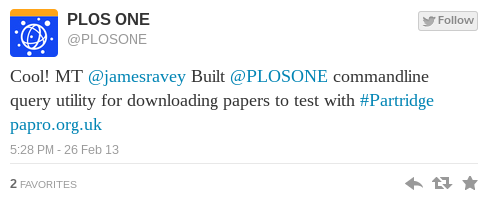
\includegraphics[width=\textwidth]{images/evaluation/plostweet.png}
\caption{Tweet from PLOSOne regarding development on Partridge}
\label{fig:plostweet}
\end{figure}

The project has also attracted the attention of the wider scientific community
on the internet, most notably the open access journal PLOSOne, from which many
of the papers used in Partridge were sourced. During the implementation of
Partridge, I constantly updated my Twitter account with news about my
progress. Figure \ref{fig:plostweet} shows one of the positive reactions to
work I was carrying out on the paper preprocessor.


\section{ Limitations and Potential Improvements }

Despite the great achievements and impact of Partridge, a few limitations and
imperfections have emerged during the course of the project. Many of these
limitations stem from incorrect estimation of the difficulty and scale
of the AI and NLP-based tasks within the system and most of them could be
improved or resolved all together if more time was available to work on the
project.

\subsection{ Paper Classifiers}

Due to the strict time restrictions, two of the paper preprocessor modules: the
result and subject classifiers could not be implemented. These were supposed to
add the ability to filter experimental papers by result: positive or negative
and filter papers by topic: e.g. Physics, Biology, Maths. After the completion
of the paper type classifier, the project deadline was only a few weeks away
and with the dissertation write-up looming, I decided it would be foolish to
start working on further classifier behaviour.

Given my experience with the paper type classifier, adding the new classifiers
for result and topic should be fairly simple if I followed the same process:
determining which features would be the most effective for discriminating
between the data classes and then training and comparing a few different
supervised learning algorithms using the Partridge corpus. A number of papers
that could be reviewed to help with feature selection and training for these
tasks have been suggested to me for review at a later date.

\subsection{ SAPIENTA }

Whilst SAPIENTA is an excellent piece of research in itself and provides
fascinating insights and implications into the makeup of scientific literature,
Dr Liakata concedes that it is purely an experimental system and was not
intended for large scale analysis of batches of papers in the way that it is
utilised by Partridge. During the development of the paper type classifier,
there were several short delays when the SAPIENTA server stopped working and
had to be restarted. For this reason, it took several weeks to collect enough data for machine
learning. 

Unfortunately, SAPIENTA is not scheduled for improvement work until the summer
and that means that Partridge's paper preprocessor is still not very
scalable. If further work to Partridge is carried out, I hope to improve the
accuracy of the Python SAPIENTA implementation to be comparable with the
current, experimental version of the system and run paper annotations locally
on the Partridge server.

\subsection{ Scalability }

Aside from the underlying issues with SAPIENTA, some of the other Partridge
subsystems may suffer from scalability issues when faced with a large volume of
users. 

Partridge currently resides on a single server machine which runs separate
database server, web server and paper preprocessor tasks. This configuration
has been effective during Partridge's development and remains effective at
present. However, if the volume of users increased significantly, a single
server machine may not offer the processing power or storage capability
required. If this becomes an issue, the database, web server and paper
preprocessor systems could all be moved to separate physical machines and
communicate over a local network.

The paper preprocessor application is also currently single threaded, only
processing one paper at a time. If more time had been available, the
preprocessing module would have been modified to use parallel processing when
processing each paper, allowing uploaded papers to be added to the database more
quickly.

\subsection{ Recommendation Engine}

During the course of the project, it quickly became clear that there would
not be time to implement a recommendation engine as originally hoped. Such a
system would need to collect data from users and the papers that they looked at
and correlate it with papers stored in the corpus that the user may be
interested in viewing. Although there wasn't time to build this feature during
the project, I certainly think it is more than feasible. 

One possible solution would be to use features such as a paper's CoreSC makeup
to build a user profile and then use a k-Nearest Neighbours algorithm to select
papers that have similar features to the user's preferences. Given the
opportunity, I would have liked to have spent a significant amount of time
investigating possible techniques and implementing a recommendation system
since this would offer a huge boost in Partridge's utility.

\section{ Further Research }

Partridge already fulfills many of its objectives and has also had a sizeable
impact on the research community. However,  during implementation, a number of
topics for further research have also been uncovered.

Towards the end of the project, I was given the opportunity to submit an
overview of Partridge as an academic research paper as part of the proceedings
for the BCS AI Conference being held in December 2013. This is an excellent
opportunity to expose Partridge to potential researchers who may be interested
in examining some of the Natural Language Processing and Artificial
Intelligence techniques employed in the project.

The relationship between a paper's  CoreSC makeup and its type has a lot of
potential for further research. During the development of Partridge, this
relationship was only tested using Research, Review and Case Study papers since
there were a large number such papers published in open access journals,
available for analysis. From the analysis in Section
\ref{sec:evaluaton_learners}, it is clear that a paper's CoreSC makeup can be
very effective in determining which of these three classes it belongs to. The
most discriminative features were specifically Background, Method and
Motivation. However, this relationship was only tested with the three paper
possible types listed above. Further work could be conducted to discern whether
the correlation between CoreSC makeup and paper type holds for other classes of
document and whether the most discriminative CoreSC labels remain the same for
a larger number of paper types.

\section{ Summary }

This chapter has discussed the achievements arising from the Partridge project:
the design and implementation of the paper preprocessor and the integrated
Artificial Intelligence; lessons learnt from developing Partridge's HTML5
interface and considerations needed to help users to understand complicated
applications; professional and personal development through my relationship
with my supervisors. Wider impacts of Partridge include a growing number of
users and interest from one of the larger research journals that Partridge
indexes.

Some of the limitations of Partridge are discussed above. These include the
additional paper classifiers which were omitted due to time constraints,
underlying problems with SAPIENTA and scalability in general. Future
development will deal with the issue of adding a recommendation engine to the
system and how this could be implemented.

Moreover, the possibility of further research into the relationship between
CoreSC and paper type is explored and I am hoping that my submission to the BCS
AI conference inspires others to carry out research in this area. 

I have thoroughly enjoyed working on Partridge and feel that this project has
developed my ability to apply machine learning algorithms to practical
applications and my professional praxis. I hope to continue to develop
Partridge into a useful and widely used research tool and am also
greatly looking forward to submitting my paper to the BCS AI Conference and
continuing my professional collaboration with Dr Clare and Dr Liakata. 
